% Practice Test 05 — Oklahoma Edition
% Questions: 30 (25 MC + 5 SA)
% Generated by scripts/generate_practice_tests.py

\begin{practiceQuestion}{1-3-q04}{mc}
\begin{questionText}
Bananas cost a fixed price per pound. The table shows the relationship. What is $k$?

\begin{center}
\begin{tabular}{|c|c|}
\hline \textbf{Pounds} & \textbf{Cost (\$)} \\ \hline $2$ & $\$1.30$ \\ $5$ & $\$3.25$ \\ $8$ & $\$5.20$ \\ \hline
\end{tabular}
\end{center}
\end{questionText}
\choiceA{$\$0.55$ per pound}
\choiceB{$\$0.65$ per pound}
\choiceC{$\$1.30$ per pound}
\choiceD{$\$1.54$ per pound}
\correctAnswer{B}
\explanation{$k = \frac{1.30}{2} = 0.65$. Check: $\frac{3.25}{5} = 0.65$ and $\frac{5.20}{8} = 0.65$. Bananas cost $\$0.65$ per pound.}
\end{practiceQuestion}

\begin{practiceQuestion}{1-6-q15}{mc}
\begin{questionText}
A car uses $3$ gallons of gas every $87$ miles. How many gallons does it need for a $435$-mile trip?
\end{questionText}
\choiceA{$10$}
\choiceB{$12$}
\choiceC{$15$}
\choiceD{$18$}
\correctAnswer{C}
\explanation{$\frac{3}{87} = \frac{x}{435}$. Cross-multiply: $87x = 1{,}305$, so $x = 15$ gallons.}
\end{practiceQuestion}

\begin{practiceQuestion}{1-7-q06}{mc}
\begin{questionText}
A map uses a scale of $1 : 10{,}000$. Two cities are $5$ cm apart on the map. What is the actual distance?
\end{questionText}
\choiceA{$50$ m}
\choiceB{$500$ m}
\choiceC{$5{,}000$ m}
\choiceD{$50{,}000$ m}
\correctAnswer{B}
\explanation{Multiply: $5 \times 10{,}000 = 50{,}000$ cm $= 500$ m.}
\end{practiceQuestion}

\begin{practiceQuestion}{2-1-q24}{sa}
\begin{questionText}
$0.5\%$ of $800$ is what number?
\end{questionText}
\correctAnswer{$4$}
\explanation{$0.5\% = 0.005$. Multiply: $0.005 \times 800 = 4$.}
\end{practiceQuestion}

\begin{practiceQuestion}{2-4-q27}{gmc}
\begin{questionText}
The table shows the cost and selling price of four items. Which item has the greatest percent markup?

\begin{center}
\begin{tabular}{|l|c|c|}
\hline
\textbf{Item} & \textbf{Cost} & \textbf{Selling Price} \\
\hline
Hat & $\$8$ & $\$14$ \\
\hline
Scarf & $\$12$ & $\$18$ \\
\hline
Gloves & $\$6$ & $\$12$ \\
\hline
Belt & $\$15$ & $\$24$ \\
\hline
\end{tabular}
\end{center}
\end{questionText}
\choiceA{Hat}
\choiceB{Scarf}
\choiceC{Gloves}
\choiceD{Belt}
\correctAnswer{C}
\explanation{Hat: $(14-8)/8 = 75\%$. Scarf: $(18-12)/12 = 50\%$. Gloves: $(12-6)/6 = 100\%$. Belt: $(24-15)/15 = 60\%$. Gloves has the greatest markup at $100\%$.}
\end{practiceQuestion}

\begin{practiceQuestion}{2-7-q16}{mc}
\begin{questionText}
An estimate has a percent error of $0\%$. What does this mean?
\end{questionText}
\choiceA{The estimate was very close}
\choiceB{The estimate was exactly correct}
\choiceC{The actual value was $0$}
\choiceD{There was no actual value to compare}
\correctAnswer{B}
\explanation{A $0\%$ percent error means the estimated value equals the actual value exactly.}
\end{practiceQuestion}

\begin{practiceQuestion}{2-8-q10}{mc}
\begin{questionText}
Compared to a bank, a credit union typically offers:
\end{questionText}
\choiceA{Higher fees and higher interest rates on loans}
\choiceB{No savings accounts}
\choiceC{Lower fees and is owned by its members}
\choiceD{Government-backed stock investments}
\correctAnswer{C}
\explanation{Credit unions are member-owned and often charge lower fees than banks.}
\end{practiceQuestion}

\begin{practiceQuestion}{3-1-q28}{gmc}
\begin{questionText}
Look at the number line. Which point has the greatest absolute value?

\begin{center}
\begin{tikzpicture}
  \draw[thick,->] (-6.5,0) -- (6.5,0);
  \foreach \x in {-6,...,6} \draw (\x,0.1) -- (\x,-0.1) node[below] {$\x$};
  \fill[funRed] (-5,0) circle (4pt) node[above=6pt] {W};
  \fill[funBlue] (2,0) circle (4pt) node[above=6pt] {X};
  \fill[funGreen] (-1,0) circle (4pt) node[above=6pt] {Y};
  \fill[funOrange] (4,0) circle (4pt) node[above=6pt] {Z};
\end{tikzpicture}
\end{center}
\end{questionText}
\choiceA{W}
\choiceB{X}
\choiceC{Y}
\choiceD{Z}
\correctAnswer{A}
\explanation{$|W| = |-5| = 5$, $|X| = 2$, $|Y| = 1$, $|Z| = 4$. Point W has the greatest absolute value at $5$.}
\end{practiceQuestion}

\begin{practiceQuestion}{4-1-q13}{mc}
\begin{questionText}
A rectangle has length $2x + 3$ and width $4$. Which expression gives its perimeter?
\end{questionText}
\choiceA{$8x + 12$}
\choiceB{$2x + 7$}
\choiceC{$4x + 14$}
\choiceD{$8x + 6$}
\correctAnswer{C}
\explanation{Perimeter $= 2(\text{length} + \text{width}) = 2(2x + 3 + 4) = 2(2x + 7) = 4x + 14$.}
\end{practiceQuestion}

\begin{practiceQuestion}{4-2-q01}{mc}
\begin{questionText}
Which pair of terms are like terms?
\end{questionText}
\choiceA{$3x$ and $3y$}
\choiceB{$5m$ and $-2m$}
\choiceC{$4n$ and $4n^2$}
\choiceD{$7$ and $7x$}
\correctAnswer{B}
\explanation{Like terms have the same variable raised to the same power. $5m$ and $-2m$ both have the variable $m$ to the first power.}
\end{practiceQuestion}

\begin{practiceQuestion}{5-3-q03}{mc}
\begin{questionText}
What is the first step to solve $5(x + 2) = 35$ using the ``divide first'' method?
\end{questionText}
\choiceA{Subtract $2$ from both sides}
\choiceB{Distribute $5$ to get $5x + 10 = 35$}
\choiceC{Divide both sides by $5$}
\choiceD{Subtract $5$ from both sides}
\correctAnswer{C}
\explanation{The ``divide first'' method divides both sides by $5$: $x + 2 = 7$.}
\end{practiceQuestion}

\begin{practiceQuestion}{5-4-q08}{mc}
\begin{questionText}
A recipe calls for $\dfrac{3}{4}$ cup of sugar per batch. You already used $\dfrac{1}{2}$ cup. You have $2\dfrac{3}{4}$ cups total. The equation $\dfrac{3}{4}b + \dfrac{1}{2} = 2\dfrac{3}{4}$ finds how many more batches $b$ you can make. What is $b$?
\end{questionText}
\choiceA{$b = 3$}
\choiceB{$b = 4$}
\choiceC{$b = 2$}
\choiceD{$b = 3\dfrac{2}{3}$}
\correctAnswer{A}
\explanation{Subtract $\frac{1}{2}$: $\frac{3}{4}b = 2\frac{1}{4} = \frac{9}{4}$. Multiply by $\frac{4}{3}$: $b = \frac{9}{4} \times \frac{4}{3} = 3$.}
\end{practiceQuestion}

\begin{practiceQuestion}{5-5-q18}{mc}
\begin{questionText}
Solve $-x + 9 \leq 15$.
\end{questionText}
\choiceA{$x \leq -6$}
\choiceB{$x \geq 6$}
\choiceC{$x \geq -6$}
\choiceD{$x \leq 6$}
\correctAnswer{C}
\explanation{Subtract $9$: $-x \leq 6$. Multiply by $-1$ and flip: $x \geq -6$.}
\end{practiceQuestion}

\begin{practiceQuestion}{5-6-q29}{gsa}
\begin{questionText}
Solve $-3x + 9 > 0$. Then graph the solution on the number line below by describing the circle type and shading direction.

\begin{center}
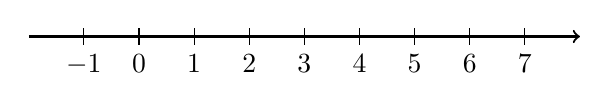
\begin{tikzpicture}[scale=0.7]
  \draw[thick,->] (-2,0) -- (8,0);
  \foreach \x in {-1,...,7} \draw (\x,0.15) -- (\x,-0.15) node[below] {$\x$};
\end{tikzpicture}
\end{center}
\end{questionText}
\correctAnswer{$x < 3$; open circle at $3$, shade left}
\explanation{Subtract $9$: $-3x > -9$. Divide by $-3$ and flip: $x < 3$. Open circle at $3$, shade left.}
\end{practiceQuestion}

\begin{practiceQuestion}{6-2-q17}{mc}
\begin{questionText}
A map uses $1$ cm $= 60$ km. You redraw it at $1$ cm $= 20$ km. A triangle on the original has an area of $4$ cm$^2$. What is its area on the new map?
\end{questionText}
\choiceA{$12$ cm$^2$}
\choiceB{$16$ cm$^2$}
\choiceC{$36$ cm$^2$}
\choiceD{$48$ cm$^2$}
\correctAnswer{C}
\explanation{Scale ratio: $\frac{60}{20} = 3$. Area scales by $3^2 = 9$. New area: $4 \times 9 = 36$ cm$^2$.}
\end{practiceQuestion}

\begin{practiceQuestion}{6-3-q08}{mc}
\begin{questionText}
Which set of conditions produces exactly one triangle?
\end{questionText}
\choiceA{Three angles: $40°$, $60°$, $80°$}
\choiceB{One side: $5$ cm}
\choiceC{Three sides: $3$ cm, $5$ cm, $7$ cm}
\choiceD{Two sides: $4$ cm and $6$ cm}
\correctAnswer{C}
\explanation{Three valid side lengths (SSS) with the triangle inequality satisfied produce exactly one unique triangle. AAA gives many, and knowing only one or two side lengths is not enough.}
\end{practiceQuestion}

\begin{practiceQuestion}{6-4-q08}{mc}
\begin{questionText}
You know two angles ($50°$ and $70°$) and the side between them is $8$ cm. What triangle condition is this?
\end{questionText}
\choiceA{SSS}
\choiceB{SAS}
\choiceC{ASA}
\choiceD{AAS}
\correctAnswer{C}
\explanation{Two angles and the included side is the ASA (Angle-Side-Angle) condition.}
\end{practiceQuestion}

\begin{practiceQuestion}{6-5-q25}{sa}
\begin{questionText}
A square pyramid has a base edge of $8$ cm. It is sliced parallel to the base halfway up. Is the cross-section larger, smaller, or the same size as the base?
\end{questionText}
\correctAnswer{Smaller than the base}
\explanation{A horizontal cut parallel to the base of a pyramid produces a similar shape that is smaller than the base. Halfway up, the cross-section is a $4$ cm square (half the edge length).}
\end{practiceQuestion}

\begin{practiceQuestion}{6-6-q02}{mc}
\begin{questionText}
Two angles are complementary. One angle is $27°$. What is the other angle?
\end{questionText}
\choiceA{$53°$}
\choiceB{$63°$}
\choiceC{$73°$}
\choiceD{$153°$}
\correctAnswer{B}
\explanation{Complementary angles sum to $90°$. $90° - 27° = 63°$.}
\end{practiceQuestion}

\begin{practiceQuestion}{7-4-q10}{mc}
\begin{questionText}
A figure is made of a trapezoid with parallel sides $6$ cm and $10$ cm, and height $4$ cm. Which expression gives its area?
\end{questionText}
\choiceA{$6 \times 10 \times 4$}
\choiceB{$\frac{1}{2} \times 6 \times 10$}
\choiceC{$\frac{1}{2} \times (6 + 10) \times 4$}
\choiceD{$(6 + 10) \times 4$}
\correctAnswer{C}
\explanation{Area of a trapezoid $= \frac{1}{2}(b_1 + b_2) \times h = \frac{1}{2}(6 + 10) \times 4 = 32$ cm$^2$.}
\end{practiceQuestion}

\begin{practiceQuestion}{7-5-q10}{mc}
\begin{questionText}
A cube has a surface area of $54$ cm$^2$. What is the area of one face?
\end{questionText}
\choiceA{$6$ cm$^2$}
\choiceB{$9$ cm$^2$}
\choiceC{$18$ cm$^2$}
\choiceD{$27$ cm$^2$}
\correctAnswer{B}
\explanation{A cube has $6$ identical faces. Area of one face $= 54 \div 6 = 9$ cm$^2$.}
\end{practiceQuestion}

\begin{practiceQuestion}{7-6-q18}{mc}
\begin{questionText}
A trapezoidal prism has a trapezoidal base with parallel sides $4$ cm and $6$ cm, height $3$ cm, and the prism length is $10$ cm. What is its volume?
\end{questionText}
\choiceA{$60$ cm$^3$}
\choiceB{$120$ cm$^3$}
\choiceC{$150$ cm$^3$}
\choiceD{$180$ cm$^3$}
\correctAnswer{C}
\explanation{$B = \frac{1}{2}(4 + 6) \times 3 = 15$ cm$^2$. $V = 15 \times 10 = 150$ cm$^3$.}
\end{practiceQuestion}

\begin{practiceQuestion}{8-1-q11}{mc}
\begin{questionText}
A survey of $200$ randomly selected adults found that $60\%$ prefer coffee over tea. If the city has $50{,}000$ adults, about how many prefer coffee?
\end{questionText}
\choiceA{$12{,}000$}
\choiceB{$20{,}000$}
\choiceC{$30{,}000$}
\choiceD{$60{,}000$}
\correctAnswer{C}
\explanation{$60\%$ of $50{,}000 = 0.60 \times 50{,}000 = 30{,}000$.}
\end{practiceQuestion}

\begin{practiceQuestion}{8-3-q08}{mc}
\begin{questionText}
The dot plots for two classes overlap significantly. The difference in their means is $2$ points, and both have a MAD of $6$. What can you conclude?
\end{questionText}
\choiceA{The classes are very different}
\choiceB{The difference in means is meaningful}
\choiceC{The difference in means is small relative to the variability}
\choiceD{You cannot compare the classes}
\correctAnswer{C}
\explanation{The difference ($2$) is much smaller than the MAD ($6$), so the difference is not very meaningful — there is a lot of overlap.}
\end{practiceQuestion}

\begin{practiceQuestion}{8-4-q30}{gsa}
\begin{questionText}
The table shows test scores for two science classes.

\begin{center}
\begin{tabular}{|l|c|c|c|c|c|c|c|c|c|c|}
\hline
\textbf{Class A} & $60$ & $65$ & $70$ & $75$ & $80$ & $85$ & $90$ & $95$ & & \\
\hline
\textbf{Class B} & $72$ & $74$ & $76$ & $78$ & $80$ & $82$ & $84$ & $86$ & & \\
\hline
\end{tabular}
\end{center}

Find the mean, median, and range for each class. Which class performed more consistently?
\end{questionText}
\correctAnswer{Both means $= 77.5$; both medians $= 77.5$; Class A range $= 35$, Class B range $= 14$. Class B is more consistent.}
\explanation{Class A: mean $= \frac{620}{8} = 77.5$, median $= \frac{75+80}{2} = 77.5$, range $= 95 - 60 = 35$. Class B: mean $= \frac{632}{8} = 79$, median $= \frac{78+80}{2} = 79$, range $= 86 - 72 = 14$. Class B has a much smaller range, so its scores are more consistent.}
\end{practiceQuestion}

\begin{practiceQuestion}{8-5-q02}{mc}
\begin{questionText}
Which of the following is true about the leaves in a stem-and-leaf plot?
\end{questionText}
\choiceA{Leaves are listed in random order}
\choiceB{Leaves are listed in order from least to greatest}
\choiceC{Each leaf represents the tens digit}
\choiceD{Leaves are always single digits from $1$ to $9$}
\correctAnswer{B}
\explanation{Leaves must be arranged in order from least to greatest so the data is easy to read.}
\end{practiceQuestion}

\begin{practiceQuestion}{8-7-q26}{gmc}
\begin{questionText}
The frequency table shows the number of books students read last month.

\begin{center}
\begin{tabular}{|c|c|}
\hline
\textbf{Books Read} & \textbf{Frequency} \\
\hline
$0$--$2$ & $6$ \\
\hline
$3$--$5$ & $14$ \\
\hline
$6$--$8$ & $8$ \\
\hline
$9$--$11$ & $2$ \\
\hline
\end{tabular}
\end{center}

What percent of students read $3$ or more books?
\end{questionText}
\choiceA{$46.7\%$}
\choiceB{$73.3\%$}
\choiceC{$80\%$}
\choiceD{$20\%$}
\correctAnswer{C}
\explanation{Total: $6+14+8+2 = 30$. Read $3+$: $14+8+2 = 24$. Percent: $\frac{24}{30} = 80\%$.}
\end{practiceQuestion}

\begin{practiceQuestion}{9-4-q24}{sa}
\begin{questionText}
Create a non-uniform probability model for a spinner with $3$ sections (A, B, C) where A is twice as likely as B, and C has the same probability as B. Write the probability of each section.
\end{questionText}
\correctAnswer{$P(A) = \frac{1}{2}$, $P(B) = \frac{1}{4}$, $P(C) = \frac{1}{4}$}
\explanation{Let $P(B) = x$. Then $P(A) = 2x$ and $P(C) = x$. Total: $2x + x + x = 4x = 1$, so $x = \frac{1}{4}$. $P(A) = \frac{1}{2}$, $P(B) = P(C) = \frac{1}{4}$.}
\end{practiceQuestion}

\begin{practiceQuestion}{9-6-q13}{mc}
\begin{questionText}
Two coins are flipped. What is the probability of getting at least one head?
\end{questionText}
\choiceA{$\frac{1}{4}$}
\choiceB{$\frac{1}{2}$}
\choiceC{$\frac{3}{4}$}
\choiceD{$1$}
\correctAnswer{C}
\explanation{At least one head: HH, HT, TH — that is $3$ out of $4$. $P = \frac{3}{4}$. Or: $1 - P(\text{no heads}) = 1 - \frac{1}{4} = \frac{3}{4}$.}
\end{practiceQuestion}

\begin{practiceQuestion}{9-7-q11}{mc}
\begin{questionText}
A bag has $3$ red and $7$ blue marbles. To simulate drawing one marble, you could use random digits $0$--$9$. Which digits would represent red?
\end{questionText}
\choiceA{$0, 1, 2$}
\choiceB{$0, 1, 2, 3$}
\choiceC{$0, 1, 2, 3, 4, 5, 6$}
\choiceD{$7, 8, 9$}
\correctAnswer{A}
\explanation{Red has a $\frac{3}{10}$ probability. Using $3$ digits ($0, 1, 2$) out of $10$ gives $\frac{3}{10} = 30\%$.}
\end{practiceQuestion}
